\documentclass[../sparc.tex]{subfiles}
\graphicspath{{\subfix{../images/}}}
\begin{document}

%%%%%%%%%%%%%%%%%%%%%%%%%%%%%%%%%%%%%%%%%%%%%%%%%%%%%%%%%%%%%%%%%%%%%%%%%%%%%%%%
\section{Building Electric Circuits}

It would be hard to talk about modern digital circuitry without mention a
\emph{micro-controller} -- it is a ``brain'' of many systems that we interact
with each day.

A micro-controller is a simple and usually quite cheap embedded computer often
built to solve one task.  Micro-controllers are in control (pun intended) of
many modern household appliances, children toys, electronic musical instruments
and factory robots; 3D-printers and other CNCs are built upon micro-controllers.

We will be working with Arduino platform that is widely available and provides
convenient interface for the practical application and programming.

Its appearance may wary depending on the model; you can find a photo of one of
the popular Arduino model called ``Arduino UNO'' on
fig. \ref{fig:arduino-uno-r3}.

\begin{figure}[ht]
  \centering
  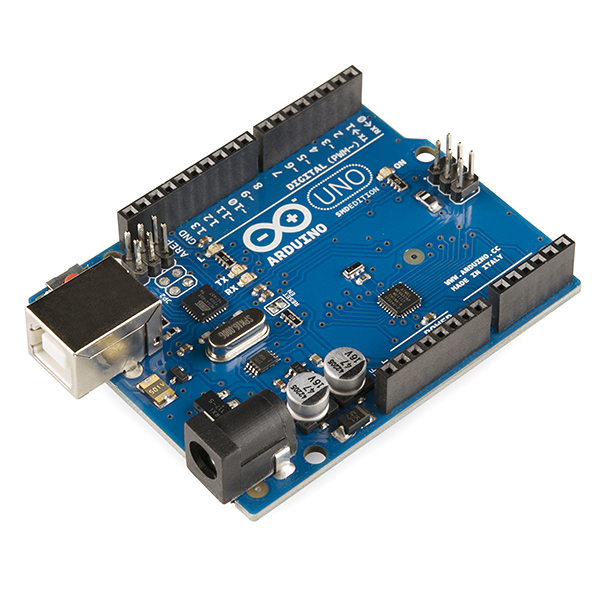
\includegraphics[width=12cm]{Arduino_Uno_-_R3}
  \caption{Micro-controller platform ``Arduino UNO'' R3.}
  \label{fig:arduino-uno-r3}
\end{figure}

We will discuss Arduino usage and programming in the chapter
\ref{chapter:dialogues-with-computer}.  Meanwhile we will use Arduino simply as
the voltage source in the place of battery in our circuits.

As shown on fig. \ref{fig:arduino-uno-r3} Arduino has special connectors that
are called \emph{ports} that allow to connect external components and wires to
the board.  Some ports are numbered as 0, 1, 2 etc. -- those are \emph{digital
ports}.  Also you can find ports labeled as ``A0'', ``A1'', ``A2'' etc. -- and
they are called \emph{analog ports}.  We won't be using digital and analog ports
in this chapter as we will need to write some program for our micro-controller
to work with them; and that's a topic for another chapter.

Now please note two Arduino ports labeled as ``GND'' and ``5V''.

``GND'' means ``Ground'' -- this is a port that always has 0V on it.  ``5V'' is
always have 5V as you probably already guessed.

Let's build an electric circuit with a resistor and an LED shown on
fig. \ref{fig:electronics-arduino-circuit-00}.

\begin{figure}[ht]
  \centering
  \begin{circuitikz}
    \draw (3.5, 0) node[
      dipchip,
      num pins=2,
      external pins width=0.0,
      no topmark,
      hide numbers,
      xscale = 2.5,
      yscale = 2.5](C1){Arduino};
    \node [above left, font=\small] at (C1.bpin 1) {5V};
    \node [above right, font=\small] at (C1.bpin 2) {GND};
    \draw
    (C1.bpin 1) to[short]
    (0, 0) to[short]
    (0, 4) to[resistor, l=$R_1$] (3, 4)
    (3, 4) to[full led, l=LED] (7, 4)
    (7, 4) to[short]
    (7, 0) to[short]
    (C1.bpin 2);
  \end{circuitikz}
  \caption{A circuit with a resistor, an LED and Arduino.}
  \label{fig:electronics-arduino-circuit-00}
\end{figure}

\end{document}
